\documentclass[10pt]{beamer}
\usetheme{metropolis}           % Use metropolis theme
\usepackage{graphicx}
\usepackage{amsmath}
\title{Crop yield prediction - A machine learning based approach}
\date{\today}
\author{Prajna Kandarpa}
\institute{University of Waterloo}
\begin{document}
  \maketitle
  % \begin{frame}{terminology}
  % 	\begin{itemize}
  % 		\item \textsc{crop yield prediction (CYP)}
  % 		\item \textsc{yield potential (Yp)} - hypothetical yield under controlled environments with no pests, diseases and adequate rainfall
  % 		\item \textsc{yield gap} - difference between yield potential and current average farm yields
  % 	\end{itemize}
  % \end{frame}
  \section{why should we predict crop yields?}
  \begin{frame}{CYP Uses}
  	\begin{itemize}
  		\item Urgent need for crop yield increase to sustain increasing global population \cite{Lobell2010}
  		\item \textbf{Crop yield predictions aim to reduce yield gap}
  		\item Help inform governmental policies and achieve food security
  		\item Crop yield varies geospatially and temporally in a non-linear fashion (duh)
  		\item \emph{curious trend observed globally - most crop yields tend to plateau at 70-80\% of Yp at regional and national levels}
  	\end{itemize}
  \end{frame}
  \section{Literature review}
  \begin{frame}{Status Quo}
  	\textbf{How do current methods work?}
  	\begin{itemize}
		\item{advanced dynamic models of crop production and socio-economic factors.}
	    	\begin{itemize}
	    		\item CERES-Wheat, CERES-Maize, CERES-Barley, SOYGRO for legumes, AFRCWHEAT2 \cite{SJAR4439}
    		\end{itemize}
		\item use decades of research on crop physiology and reproduction, agronomy, and soil science, among other disciplines
		\item Need to collect data through multi-disciplinary experiments
		% \item not always viable for all countries
		\item Research that seeks to emulate model results using statistical and ML models - goal of this project
	\end{itemize}
  \end{frame}
  \section{Data Sources and Preprocessing}
  \begin{frame}{Crop selection}
  	Rice, Maize - Subset of data for a single district(region)
  	\begin{center}
  	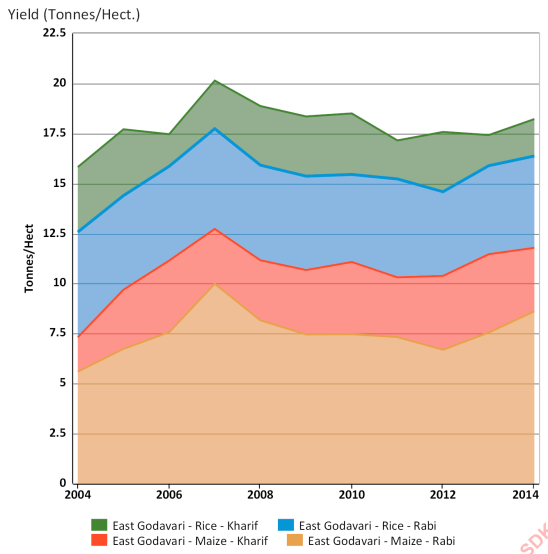
\includegraphics[width=0.55\textwidth]{ego_rice.png}
  	\end{center}
  \end{frame}
  \begin{frame}{Data Sources and Preprocessing}
	\textbf{Data Sources}
  	\begin{itemize}
  		% \item Need to combine data from multiple sources
  		% \item currently have weather and crop yield data for India
  		\item weather data from 1872-2014 (regional precipitation levels for the country of India)
  		\item Crop yield data from 1959-2014
  		% \item http://knoema.com/ICPS2015/crop-production-statistics-of-india-1999-2014?regionId=IN
  		% \item about 
  	\end{itemize}
  \end{frame}

  \begin{frame}{Feature Selection}
  	\textbf{Weather - regional resolution}
  	2 agricultural seasons in India - Kharif and Rabi
  	\begin{itemize}	
  		\item precipitation levels
  		\item temperature
  		\item humidity
  		% \item both these features are grouped into a discrete number of states 
  		% \item temperature is hard to bin in a way that captures its variability in tropical regions
  		% \item 
  	\end{itemize}
  	\textbf{Physiographic data}
  	\begin{itemize}
  		\item area under cultivation 
  		\item irrigation levels
  	\end{itemize}
  \end{frame}
  \begin{frame}{Prediction Accuracy}
  	\textbf{Output = seasonal crop yield at regional level}
  	\begin{itemize}
  		% \item compare with estimates published by the Government of India.
  		% \item \href{http://eands.dacnet.nic.in/Advance_Estimate/2ndAd18022015ENG.pdf}{Link here}
  		\item Standard regression error measures
  		\item Root Mean Squared Error (RMSE)
  		% \item Mean Absolute Error (MAE)
  		\item Mean Absolute Percentage Error (MAPE)
  	\end{itemize}
  \end{frame}
  \section{Analysis Methods}
  \begin{frame}{Machine learning for CYP}
  	\emph{machine learning is statistics minus any checking of models and assumptions} - Brian D. Ripley
  	\begin{itemize}
  		\item can we achieve results similar to advanced crop models using fewer variables?
  		\item ML approaches are data driven - require lesser understanding of the underlying physical systems
  		% \item time series prediction
  		\item analogous to financial time series forecasting
  	\end{itemize}
  \end{frame}
  \begin{frame}{Modeling Techniques}
  	Time series prediction involves measuring \emph{co-movement}

  	co-movement is a measure of correlation between covariation, detrended cross correlations with frequency, trends, seasonality and uncertainty of the data
  	
 %  	\alert{what does a model measure?}
 %  	\begin{itemize}
	% \item frequency, trends, seasonality, uncertainty, clusters
	% \item drift model - growth/decay of time series
	% \item seasonal model - cycles in the time series
	% \item uncertainty - historical volatility and implied volatility
	% \end{itemize}

	% \alert{common time series prediction models}
	\begin{itemize}
	\item Convolutional Neural Networks with 3-7 hidden layers - experiment with number of layers and number of nodes in each layer
	\item MARS - Multiple Adaptive Regressive Splines
	\item Support Vector Regression
	\end{itemize}

  \end{frame}
  \begin{frame}{Steps}
  \begin{center}
  $ \hat{y}[t+1] = f(y[t-k], ...,y[t])$
  \end{center}

  All analysis is done in R using \emph{caret}
  	\begin{enumerate}
		% \item Non homogeneous markov models have been used for rainfall modeling (daily multi site precipitation modeling)
  % 		\item Mixtures of trees - a mixture model where each mixture component has a different conditional dependence between variables
  % 		\item need to compress high dimensional weather data into a smaller number of discrete states (its still time series)
  % 		\item makes it easier to interpret the results.
  		\item Cleaned weather, yield, land datasets into a single dataframe
  		\item Pick important predictors using covariance measures
  		\item Data binning, filtering, k-fold cross validation
  		\item train all 3 models
  		\item Prediction cross validation across all evaluated models

  	\end{enumerate}
  \end{frame}
  \begin{frame}{Extras}
  	Depending on performance of NN, SVR and MARS models, build a crop recommendation tool for farmers that factors in historical performance and regional crop yields

  	Assess inferential viability of neural network by examining hidden layer outputs

  	Crop Recommendation tool requires yield prediction models for each crop
  \end{frame}
  \begin{frame}{References}
  % \te
  	\bibliography{presentation}
  	\bibliographystyle{IEEEtran}
  \end{frame}
\end{document}